\section{Делимость}

В этом параграфе мы одним махом рассмотрим все базовые свойства делимости и связанные с этим понятия. Напомню, что мы ввели обозначение $a|b$ для обозначения делимости $b$ на $a$ (равносильно $a$ делит $b$).. Формально это значит, что $b=ka$ для некоторого $k$.

\begin{thm}
Если в сумме $\sum_{i=0}^na_i$ все слагаемые делятся на $b$, то и вся сумма делится на $b$.
\end{thm}
\begin{proof}
По условию теоремы $a_i = k_i b$. Тогда
$$\sum_{i=0}^na_i = \sum_{i=0}^n bk_i = b\sum_{i=0}^n k_i$$
Последнее выражение как раз и означает, что первоначальная сумма делится на $b$, поскольку мы смогли из всей суммы вынести этот множитель за скобки.
\end{proof}

\begin{thm}
Если в сумме $\sum_{i=0}^na_i$ все слагаемые кроме одного делятся на $b$, то сумма не делится на $b$.
\end{thm}
\begin{proof}
Поскольку мы можем переставлять слагаемые как нам вздумается, будем считать, что на $b$ не делится слагаемое $a_0$, а остальные слагаемые делятся. Это значит, что $a_0 = k_0 b + r, r>0$ и для всех $i>0$ имеем $a_i=k_i b$. Тогда мы можем записать сумму в следующем виде:
$$\sum_{i=0}^na_i = k_0 b + r + \sum_{i=1}^n b k_i = b\sum_{i=0}^n k_i + r$$
Последнее есть ни что иное как деление с остатком суммы на $b$, где остаток $r>0$. Это ровно то, что требовалось доказать.
\end{proof}

\begin{exercise}
В теореме 3.14 принципиально то, что не делится на $b$ лишь одно из слагаемых, но не больше. Покажите, что если в сумме не делится на $b$ ровно два слагаемых, то сама сумма на $b$ всё же может делиться.
\end{exercise}

\begin{exercise}
Докажите, что для того, чтобы произведение $\prod_{i=0}^n a_i$ делилось на $b$, достаточно, чтобы хотя бы один из множителей $a_i$ делился на $b$. Это условие не является необходимым: покажите так же, что возможна ситуация, когда ни один из множителей не делится на $b$, но само произведение на $b$ делится.
\end{exercise}

\begin{definition}
Число называется \term{чётным}, если оно делится на 2, и \term{нечётным} в противном случае.
\end{definition}

Любое чётное число может быть представлено в виде $2k$, а нечетное в виде $2k+1$.

\begin{exercise}
Докажите, что сумма двух чётных чисел чётна, сумма двух нечётных так же чётна, а сумма чётного и нечётного нечётна. Докажите так же, что произведение нечетных чисел всегда нечетное, и что если хотя бы один из множителей чётный, то и всё произведение чётно.
\end{exercise}

Понятие чётности/нечётности вроде на первый взгляд совершенно тривиально, однако оно постоянно возникает в математике. Например, в прошлом параграфе оно нам уже встречалось, хотя мы тогда не обратили на него внимания. С новой терминологией мы можем переформулировать алгоритм возведения в степень так: если $b$~--- чётное, то $a^b = (a^{b/2})^2$, а если нечётное, то $a^b = (a^{(b-1)/2})^2 a$. Мелочь, но подобная терминология в математике и её приложениях встречается сплошь и рядом, это довольно удобно.

Используя теоремы выше мы можем легко вывести школьные <<признаки делимости>>.

\begin{example}
Для того, чтобы число делилось на 4, необходимо и достаточно, чтобы число, составленное из двух младших разрядов делилось на 4. Действительно:
$$\sum_{i=0}^\infty a_i 10^i = 100 \sum_{i = 2}^\infty a_i 10^{i-2} + (10a_1 + a_0)$$
В последнем выражении сумма слева делится на 4, поэтому для делимости всего числа на~4 по теоремам~3.13-14 необходимо и достаточно, чтобы делилось на 4 выражение $10a_1 + a_0$, а это и есть две последние цифры. Так, число 4133 не делится на 4, так как 33 не делится на 4, а число 12344 делится на четыре, так как 44 делится на 4.
\end{example}

\begin{exercise}
Докажите, что для того, чтобы число было четным, необходимо и достаточно, чтобы младший разряд числа был чётным.
\end{exercise}

\begin{exercise}
Докажите, что для того, чтобы число делилось на 5, необходимо и достаточно, чтобы младший разряд был равен 0 либо 5.
\end{exercise}

\begin{example}
Для того, чтобы число делилось на 3, необходимо и достаточно, чтобы сумма его цифр делилась на 3. Дейстивительно:
\begin{align*}
\sum_{i=0}^\infty a_i 10^i &= a_0 + (9+1)a_1 + (99+1)a_2 + \ldots\\
    &= \sum_{i=0}^\infty a_i + 9a_1 + 99a_2 + 999a_3 +\ldots \\
    &= \sum_{i=0}^\infty a_i + 3(3a_1 + 33a_2 +\ldots)
\end{align*}
Второе слагаемое всегда делится на три, поэтому для делимости всей суммы необходимо и достаточно, чтобы делилась на три сумма $\sum_{i\in\mathbb{N}} a_i$.
\end{example}

\begin{exercise}
Докажите, что для того, чтобы число делилось на 9, необходимо и достаточно, чтобы сумма его цифр делилась на 9.
\end{exercise}

\begin{example}
Можно придумать еще множество критериев подобным образом, а так же сочетая существующие критерии. Например, для того, чтобы число делилось на 6, необходимо и достаточно, чтобы оно одновременно делилось на 2 и на 3. Придумайте еще подобные критерии.
\end{example}

Как мы уже отмечали в первом параграфе, отношение делимости задаёт частичный порядок на $\mathbb{N}$. Как и прочие частичные порядки (см.\S2.2) этот порядок можно наглядно изобразить в виде диаграммы. На рисунке~3.3 изображено несколько натуральных чисел, связанных отношением делимости. Полную диаграмму делимости для чисел $\mathbb{N}$ вряд ли возможно себе вообразить, но понимание того, что числа возможно частично упорядочить таким образом (причем концептуально это ни чуть не хуже привычного упорядочивания <<больше-меньше>>, это просто еще один способ), будет необходимым для нашего следующего определения.

\begin{figure}[h]
\centering
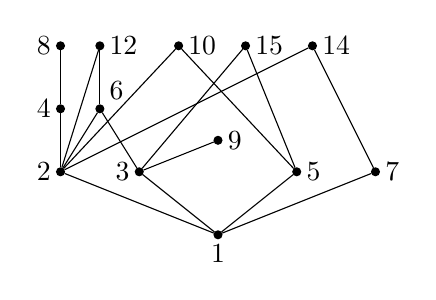
\begin{tikzpicture}
\def\point{node [circle, draw, fill, inner sep = 0, minimum size = .1cm] }
\draw (0, 0) \point (p1) {};
\draw (-2cm, .8cm) \point (p2) {};
\draw (-1cm, .8cm) \point (p3) {};
\draw (-2cm, 1.6cm) \point (p4) {};
\draw (1cm, .8cm) \point (p5) {};
\draw (-1.5cm, 1.6cm) \point (p6) {};
\draw (2cm, .8cm) \point (p7) {};
\draw (-2cm, 2.4cm) \point (p8) {};
\draw (0, 1.2cm) \point (p9) {};
\draw (-.5cm, 2.4cm) \point (p10) {};
\draw (-1.5cm, 2.4cm) \point (p12) {};
\draw (1.2cm, 2.4cm) \point (p14) {};
\draw (.35cm, 2.4cm) \point (p15) {};

\draw (p1) -- (p2);
\draw (p1) -- (p3);
\draw (p1) -- (p5);
\draw (p1) -- (p7);
\draw (p2) -- (p4);
\draw (p2) -- (p6);
\draw (p3) -- (p6);
\draw (p4) -- (p8);
\draw (p3) -- (p9);
\draw (p2) -- (p10);
\draw (p5) -- (p10);
\draw (p2) -- (p12);
\draw (p6) -- (p12);
\draw (p2) -- (p14);
\draw (p7) -- (p14);
\draw (p3) -- (p15);
\draw (p5) -- (p15);

\node [below] at (p1) {1};
\node [left] at (p2) {2};
\node [left] at (p3) {3};
\node [left] at (p4) {4};
\node [right] at (p5) {5};
\node [above right] at (p6) {6};
\node [right] at (p7) {7};
\node [left] at (p8) {8};
\node [right] at (p9) {9};
\node [right] at (p10) {10};
\node [right] at (p12) {12};
\node [right] at (p14) {14};
\node [right] at (p15) {15};

\end{tikzpicture}
\caption{Частичный порядок, заданный отношением делимости}
\end{figure}

Напомню, что в~\S~2.2 мы ввели понятие точных нижних и точных верхних граней для частично упорядоченных множеств и обозначили это как $\inf$ и $\sup$ соответственно. Эти понятия можно применить и к отношению делимости:

\begin{definition}
\term{Наибольшим общим делителем (НОД)} чисел множества $S$ называется $\inf S$, а \term{наименьшим общим кратным (НОК)} $\sup S$ относительно порядка делимости.
\end{definition}

Это определение требует, видимо, расшифровки. Для простоты будем считать, что множество $S$ состоит из двух чисел $x$ и $y$, хотя всё сказанное легко обобщается на случай произвольного конечного количества чисел.

Величина $d$ называется общим делителем чисел $x$ и $y$, если одновременно $d$ делит и $x$ и $y$. Множество всех нижних граней множества $\{x, y\}$ есть на самом деле множество общих делителей этих чисел~--- это хорошо видно из рисунка. Например, нижними гранями множества $\{10, 15\}$ являются числа 1 и 5. Если взять, например, число 2, то оно будет являться нижней гранью для $\{10\}$, но поскольку оно не сравнимо с 15, нижней гранью $\{10, 15\}$ оно не является.

Можно привести такой наглядный образ: пусть из точки диаграммы $x$ вниз по линиям стекает жидкость $A$, а из точки диаграммы $y$ стекает жидкость $B$. Если опять же рассматривать пример чисел $x=10$ и $y=15$, то жидкость $A$ течет через точки 10, 2, 5 и 1, а жидкость $B$ через точки 15, 3, 5 и 1. Точки, в которых жидкости смешиваются~--- это и есть общие грани множества $\{x, y\}$, а по совместительству еще и множество общих делителей. Самая большая из таких точек есть наибольший общий делитель.

\begin{exercise}
Докажите, что наибольший общий делитель всегда определен однозначно.
\end{exercise}

Аналогично число $d$ называется общим кратным чисел $x$ и $y$, если оно делится одновременно и на $x$ и на $y$. Наименьшее из таких чисел~--- это наименьшее общее кратное, а по совместительству точная нижняя грань из всех общих кратных.

Часто в учебниках принято обозначать НОД как $\gcd$ (greatest common divisor), а НОК как $\lcm$ (least common multiplier). Нам НОК будет требоваться довольно редко, а вот для НОД мы примем другое обозначение: вместо $\gcd(x, y)$ будем писать просто $(x, y)$. На данный момент это может показаться странным и бессмысленным, но на это есть глубокая причина, которую читатель увидит в следующей главе.

\begin{definition}
Число называется \term{простым}, если имеет в точности два делителя.
\end{definition}

\begin{definition}
Число называется \term{составным}, если оно не простое.
\end{definition}

Два делителя~--- это само число и единица. Можно было бы сказать <<не имеет делителей, кроме себя и единицы>>, это было бы понятнее, но тогда такое определение распространялось бы и на саму единицу, которая в соответствии с данным определением простым числом не является. Может возникнуть вопрос: а почему не считать единицу за простое число? Быстрый ответ таков, что это просто удобнее в большинстве случаев. Более глубокий ответ будет дан в следующей главе.

\begin{definition}
Числа $x$ и $y$ называются \term{взаимопростыми}, если $(x, y) = 1$.
\end{definition}

Любое число, если оно не простое, можно представить в виде произведения некоторых других чисел. Эти числа, если они не простые, опять же можно представить в виде какого-то произведения. Например,
$$120 = 10 \cdot 12 = 2\cdot 5 \cdot 2 \cdot 6 = 2\cdot 5 \cdot 2 \cdot 2 \cdot 3$$
Таким образом, любое натуральное число мы можем представить в виде произведения простых чисел и простые числа оказываются в некотором смысле строительными блоками для всех остальных натуральных чисел. Возникает естественный вопрос: а сколько простых чисел всего? Или хотя бы их конечное число, или бесконечное? Ответ даёт следующая теорема.

\begin{Euclids}
Простых чисел бесконечно много.
\end{Euclids}
\begin{proof}
Пойдём от противного и предположим, что это не так. Пусть простых чисел всего $N$ штук. Обозначим их как ${p_i}$. Тогда число $1 + \prod_{i=1}^N p_i$ не делится ни на одно из $p_i$, и соответственно само является простым. Это противоречит тому, что простых чисел всего $N$ штук, откуда следует что простых чисел бесконечно много.
\end{proof}

Касательно разложения чисел на простые множители остаётся еще такой вопрос: а однозначное ли это разложение? То есть понятно, что оно не однозначно с точки зрения порядка сомножителей, однако сами эти эти сомножители будут ли всегда одними и теми же, или могут отличаться? Так сходу это уже не докажешь, потребуется некоторая подготовка.

Займем из далека и начнем с быстрого способа нахождения НОД, который так же носит имя Евклида. Пусть нам надо найти величину $(x, y)$. Вначале поделим с остатком $x$ на $y$:
$$x = q_0 y + r_0$$
Теперь поделим с остатком $y$ на $r_0$:
$$y = q_1 r_0 + r_1$$.
И будем продолжать этот нехитрый процесс:
$$r_0 = q_2 r_1 + r_2$$
$$r_1 = q_3 r_2 + r_3$$
$$\dots$$
Последовательность $\{r_i\}$ строго убывающая, поэтому в какой-то момент у нас эти числа поделятся без остатка:
$$r_{n-2} = q_n r_{n-1} + r_n$$
$$r_{n-1} = q_{n+1} r_n$$
Давайте покажем, что $r_n$ является НОД чисел $a$ и $b$. Из последней строчки видно, что $r_n | r_{n-1}$. Перепишем теперь предпоследнюю строчку таким образом:
$$r_{n - 2} - q_n r_{n - 1} = r_n$$
Здесь и $r_n$ и $r_{n-1}$ делятся на $r_n$, стало быть и $r_{n-2}$ обязана делиться на $r_n$. Поднимаясь еще на строчку выше, получим аналогично, что $r_n|r_{n-3}$. Продолжая процесс нужное количество шагов, мы придём в результате к тому, что $r_n|x$ и $r_n|y$.

Это доказывает, что $r_n$ является общим делителем, но не доказывает, что это делитель наибольший. Пусть $d = (x, y)$. Из первой строчки алгоритма Евклида видно, что $d|r_0$. Из второй строчки теперь можно увидеть, что $d|r_1$. Спускаясь ниже, получаем, что $d|r_n$, но $r_n$ и сам является делителем $x$ и $y$. Это доказывает, что действительно $r_n = (x, y)$.

Сам по себе этот алгоритм хоть и быстр, но нам бесполезен: мы не собираемся искать НОД чисел. Что нам интересно, так это следствия из этого алгоритма.

Перепишем предпоследний шаг алгоритма Евклида как $r_n = r_{n-2} - q_n r_{n-1}$. Поднимемся на строчку выше, и из $r_{n-3} = q_{n-1} r_{n-2} + r_{n-1}$ подставим значение $r_{n-1}$:
$$r_n = r_{n-2} - q_n(r_{n-3} - q_{n-1}r_{n-2}) = (1+q_n q_{n-1})r_{n-2} - q_n r_{n-3}$$
Поднимаясь на строчку выше, мы можем выразить $r_{n-2}$ через $r_{n-3}$ и $r_{n-4}$, после чего мы получим следующее выражение:
$$r_n = \alpha r_{n-3} + \beta r_{n-4}$$
Здесь $\alpha$ и $\beta$~--- это некоторые коэффициенты, выражающиеся через значения $q_i$. Их можно найти строго, но они нас не волнуют. На самом деле возможно тут будет и не сумма, а разность, например, $\alpha r_{n-3} - \beta r_{n-4}$ или наоборот $\beta r_{n-4} - \alpha r_{n-3}$. Мы будем считать, что один из коэффициентов может идти со знаком минус (в следующей главе мы введем отрицательные числа и нам не надо будет делать таких оговорок, но пока будем считать так).

Продолжая процесс построчно вверх по алгоритму Евклида, мы в конечном счете приходим к такому выражению:

\begin{Bezus}
$(x, y) = \lambda x + \mu y$ для любых $x$ и $y$, где $\lambda$ и $\mu$ могут содержать знак минус.
\end{Bezus}
\begin{corollary}
Если числа $x$ и $y$ взаимопросты, то найдутся такие $\lambda$ и $\mu$, что
$$\lambda x + \mu y = 1$$
\end{corollary}
\begin{corollary}
Если числа $x$ и $y$ взаимопросты, то любое число $n$ может быть представлено как
$$n = \lambda x + \mu y$$
\end{corollary}
\begin{proof}
Первое следствие элементарно, поскольку оно фуктически дублирует определение взаимной простоты $(x, y) = 1$. Второе следствие получается из первого, если умножить обе части на $n$:
$$(n\lambda) x + (n\mu) y = n$$
\end{proof}

\begin{EuclidsLemma}
Пусть $a$ и $b$ произвольные числа и $p$~--- простое число такое, что $p|ab$. Тогда либо $p|a$, либо $p|b$.
\end{EuclidsLemma}
\begin{proof}
Предположим, что $p$ не делит $a$. В этом предположении докажем, что оно обязано тогда делить $b$. Если $p$ не делит $b$, то рассуждения будут симметричны, но в отношении $a$.

Поскольку $p$ простое и не делит $a$, это значит, что оно взаимопросто с $a$. По соотношению Безу
$$\lambda p + \mu a = 1$$
Умножим это на $b$:
$$ \lambda bp + \mu ab = b$$
В левой части оба слагаемых делятся на $p$. Значит, правая часть так же должна делиться на $p$.
\end{proof}

Вот теперь мы готовы к финальному шагу.

\begin{FTA}
Любое натуральное число однозначно раскладывается на простые множители с точностью до порядка сомножителей.
\end{FTA}
\begin{proof}
Предположим, что это не так и некоторое число одновременно может быть записано как $p_1^{\alpha_1}\ldots p_n^{\alpha_n}$ и как $q_1^{\beta_1}\ldots q_n^{\beta_n}$, где $\{p_i\}$ и $\{q_j\}$ наборы различных простых чисел.

Возьмём некоторое произвольное $p_i$ из первого разложения. Лемма Евклида гарантирует нам, что $p_i$ обязано делить один из множителей $q_j^{\beta_j}$. Аналогично можно сказать, что и каждый из $q_j$ обязан делить один из множителей $p_i^{\alpha_i}$. Если учесть, что множители в одном разложении взаимопросты, то соответсвие получается взаимооднозначным. Таким образом, сами простые множители в обоих разложениях будут одинаковыми, но нам еще надо доказать, что у них будут совпадать показатели степени.

Итак, пусть теперь у нас есть два разложения $p_1^{\alpha_1}\ldots p_n^{\alpha_n}$ и $p_1^{\beta_1}\ldots p_n^{\beta_n}$ и предположим, что $\alpha_i < \beta_i$ для некоторого $i$ (неравенство может быть и в другую сторону, доказательство в этом случае аналогично). Поделим оба этих разложения на $\alpha_i$. Тогда первое разложение более вообще не будет делиться на $p_i$, а второе разложение будет на него делиться. Из этого противоречия следует, что $\alpha_i=\beta_i$, что завершает доказательство.
\end{proof}

К этому доказательству можно было бы добавить формальных деталей, так как пока оно не слишком строго. Мы покажем как это делается в следующем параграфе.

Основная теорема арифметики имеет ряд немедленных простых следствий, которые составляют следующие упражнения, обязательные для выполнения:

\begin{exercise}
Это для разминки. Пусть $a = 2^{a_1}3^{a_2}5^{a_3}\ldots p_k^{a_k}$ и $b = 2^{b_1}3^{b_2}5^{b_3}\ldots p_k^{b_k}$~--- разложения чисел на простые множители (показатели степеней могут быть нулевыми). Докажите, что
$$ab = 2^{a_1+b_1}3^{a_2+b_2}5^{a_3+b_3}\ldots p_k^{a_k+b_k}$$
$${a\over b} = 2^{a_1-b_1}3^{a_2-b_2}5^{a_3-b_3}\ldots p_k^{a_k-b_k}$$
\end{exercise}

\begin{exercise}
Пусть $a$ и $b$ опять имеют разложение на простые множители так же как в прошлом упражнении. Докажите, что
$$(a, b) = 2^{\min\{a_1, b_1\}} 3^{\min\{a_2, b_2\}}\ldots p_k^{\min\{a_k, b_k\}}$$
$$\lcm(a, b) = 2^{\max\{a_1, b_1\}} 3^{\max\{a_2, b_2\}}\ldots p_k^{\max\{a_k, b_k\}}$$
\end{exercise}

\begin{exercise}
Докажите, что $ab = (a, b) \lcm(a, b)$.
\end{exercise}

\begin{exercise}
Докажите, что число делителей числа $a$ равнаяется величие
$$(a_1 + 1)(a_2 + 1)\ldots(a_k + 1)$$
\end{exercise}

\begin{exercise}
Докажите, что отношение делимости задаёт дистрибутивную решётку на $\mathbb{N}$ (решетки рассматривались в конце~\S2.2). Для тех, кто не разобрался с понятием дистрибутивной решетки, поясню, что это равносильно доказательству двух утверждений:
$$(a, \lcm(b, c)) = (\lcm(a, b), \lcm(a, c))$$
$$\lcm(a, (b, c)) = \lcm((a, b), (a, c))$$
\end{exercise}

\begin{exercise}
Встречаются два давнишних друга и между ними происходит следующий диалог:\\
--- Привет! Как жизнь?\\
--- Ого! Давно?\\
--- Да не, сыновья еще маленькие, в школу даже не ходят.\\
--- А сколько им лет?\\
--- Произведение из возрастов равняется количеству голубей вокруг нашей скамейки.\\
--- Чего-то ничего не понятно.\\
--- Старший похож на мать.\\
--- А теперь понятно.\\
Вопрос: сколько лет сыновьям?
\end{exercise}

Конечно, эта задача из области головоломок. В следующем абзаце я привожу две подсказки, которые почти сразу дадут решение, поэтому не читайте следующий абзац, если еще самостоятельно не успели подумать.

Секрет кроется в трёх нюансах. Во-первых, то что дети не ходят в школу даёт нам понять, что им меньше семи лет. Во-вторых, фраза о том, что <<старший похож на мать>> говорит нам о том, что дети не являются близнецами. Третий нюанс самый тонкий: собеседник, который отвечает <<теперь всё понятно>> видит конкретное количество голубей, и нам достоверно известно из диалога, что он сам каким-то образом сумел понять сколько голубей вокруг лавки. То есть это число такого, что двух первых условий оказывается достаточно для именно однозначного ответа. Думайте.